A dynamical system is given as
\begin{equation}
    \begin{cases}
    \dot{x}=Ax+Bu&\\
    x(0)=x_0&
    \end{cases}
\end{equation}
where $A\in\mathbb{R}^{nxn}$, $B\in\mathbb{R}^{nxm}$, $x\in\mathbb{R}^{nx1}$ and $u\in\mathbb{R}^{mx1}$. The control signal is constrained with 
\begin{equation}
    g_i\leq u\leq h_i\quad i=1,2,\cdots,m
\end{equation}

Let's assume the system matrices as follows
\begin{equation}
    A=\begin{bmatrix}
        a_{11}& a_{12}\\
        a_{21}& a_{22}
    \end{bmatrix},\quad
    B=\begin{bmatrix}
        b_{11}\\b_{21}
    \end{bmatrix},\quad
\end{equation}
and hence, $n=2$ and $m=1$. Then,
\begin{equation}
    g\leq u\leq h
\end{equation}
and 
\begin{equation}
    L=\begin{bmatrix}
        l_{11}\\l_{21}
    \end{bmatrix}
\end{equation}
can be stated. The closed-loop matrix is obtained as,
\begin{equation}
    A+BL^T=\begin{bmatrix}
        a_{11} + b_{11}l_{11}& a_{12} + b_{11}l_{21}\\
        a_{21} + b_{21}l_{11}& a_{22} + b_{21}l_{21}\\
    \end{bmatrix}
\end{equation}
$E(L)$ is defined as follows
\begin{equation}
\begin{split}
    E(L)&=\{z|z\in\mathbb{R}^2\,and\,g\leq l_i^Tz\leq h\}\\
    &=g\leq l_{11}z_{11} + l_{21}z_{21}\leq h
\end{split}
\end{equation}
$F(L)$ is defined as follows
\begin{equation}
    F(L)=\bigcap\limits_{t\in[0,\infty]}\{(e^{A_ct})^{-1}E(L)\}
\end{equation}
where $F(L)$ is a subset of $E(L)$.
Let $K=k_1$, then 
\begin{equation}
    u=sat[(L^T-KB^TP)x]
\end{equation}
is defined. Consider 
\begin{equation}
\begin{split}
    u&=L^Tx+v\\
    &=l_{11}x_1+l_{21}x_2+v
\end{split}
\end{equation}
then the closed-loop system is 
\begin{equation}
    \dot{x}=(A+BL^T)x+Bv
\end{equation}
which is openly,
\begin{equation}
    \begin{split}
        \dot{x}_1&=(a_{11} + b_{11}l_{11})x_1+(a_{12} + b_{11}l_{21})x_2\\
        \dot{x}_2&=(a_{21} + b_{21}l_{11})x_1+(a_{22} + b_{21}l_{21})x_2
    \end{split}
\end{equation}
The derivative of the Lyapunov function $V=x^TPx$ is obtained as,
\begin{equation}
\begin{split}
    \dot{V}&=\dot{x}^TPx+x^TP\dot{x}\\
    &=((A+BL^T)x+Bv)^TPx+x^TP((A+BL^T)x+Bv)\\
    &=(v^TB^T+x^TLB^T+x^TA^T)Px+x^TP((A+BL^T)x+Bv)\\
    &=v^TB^TPx+x^TLB^TPx+x^TA^TPx+x^TPAx+x^TPBL^Tx+x^TPBv\\
    &=x^T(A^TP+PA+PBL^T+LB^TP)x+2x^TPBv
\end{split}
\end{equation}
For stability,
\begin{equation}
    2x^TPBv\leq 0
\end{equation}
is needed. Choosing $v=-RB^TPx$ gives,
\begin{equation}
    \begin{split}
        2x^TPBv&=2x^TPB(-RB^TPx)\\
        2x^TPBv&=-2x^T(PBRB^TP)x\\
        2x^TPBv&\leq 0
    \end{split}
\end{equation}
where $R=diag([r_1,r_2,\cdots,r_m])$. Therefore,
\begin{equation}
    \begin{split}
        \dot{V}&=x^T(A^TP+PA+PBL^T+LB^TP)x+2x^TPBv\\
        \dot{V}&=x^T(A^TP+PA+PBL^T+LB^TP)x-2x^T(PBRB^TP)x\\
        \dot{V}&=x^T(A^TP+PA+PBL^T+LB^TP-2PBRB^TP)x\\
        \dot{V}&=x^T(A^TP+PA+PB(L^T-RB^TP)+(L-PBR)B^TP)x
    \end{split}
\end{equation}
Solving,
\begin{equation}
    L^Tx-RB^TPx=sat[L^Tx-KB^TPx]
\end{equation}
for any diagonal $K$.
\begin{equation}
\begin{split}
    L^Tx-RB^TPx&=sat[L^Tx-KB^TPx]\\
\end{split}
\end{equation}
which is expanded as
\begin{equation}
    \begin{split}
    l_{11}x_1+l_{21}x_2-(b_{11}p_{11}r+b_{21}p_{12}r)x_1+(-b_{11}p_{12}r-b_{21}p_{22}r)x_2\\
    =sat(l_{11}x_1+l_{21}x_2-(b_{11}p_{11}k+b_{21}p_{12}k)x_1+(-b_{11}p_{12}k-b_{21}p_{22}k)x_2)
    \end{split}
\end{equation}
if $x\in E(L)$ then 
\begin{equation}
    g\leq l_{11}x_1+l_{21}x_2 \leq h
\end{equation}
but if also
\begin{equation}
    g\leq l_{11}x_1+l_{21}x_2-(b_{11}p_{11}k+b_{21}p_{12}k)x_1-(b_{11}p_{12}k+b_{21}p_{22}k)x_2\leq h
\end{equation}
then $r=k$. On the other hand, if
\begin{equation}
    l_{11}x_1+l_{21}x_2-k(b_{11}p_{11}+b_{21}p_{12})x_1-k(b_{11}p_{12}+b_{21}p_{22})x_2> h
\end{equation}
if a smaller $r$ then the term
\begin{equation}
    l_{11}x_1+l_{21}x_2-r(b_{11}p_{11}+b_{21}p_{12})x_1-r(b_{11}p_{12}+b_{21}p_{22})x_2
\end{equation}
would increase. Therefore,
\begin{equation}
    l_{11}x_1+l_{21}x_2-r(b_{11}p_{11}+b_{21}p_{12})x_1-r(b_{11}p_{12}+b_{21}p_{22})x_2=h
\end{equation}
The algorithm is given as follows:
\begin{enumerate} 
    \item Determine $\mathbb{D}$. (set of initial states)
    \item Find $L$. Control penalty $R$ in LQR is increased until $L^Tx$ satisfies
    \begin{equation}
        g\leq L^Tx\leq h
    \end{equation}
    for $x$ in $\mathbb{D}$. This can be done via
    \begin{equation}
        g\leq\max_{x\in\mathbb{D}}l_i^Tx\leq h
    \end{equation}
    If this cannot be satisfied then there is no design.
    \item Find $P$ and $c$. $P$ can be used from LQR. $c$ is obtained from
    \begin{equation}
    \begin{split}
        \sup_{x\in\mathbb{D}}x^TPx\leq c\leq \min_{\delta E(L)}x^TPx\\
        \min_{\delta E(L)}x^TPx=\min_i{\frac{g_i^2}{l_i^TP^{-1}l_i},\frac{h_i^2}{l_i^TP^{-1}l_i}}\\
    \end{split}
    \end{equation}
    If this fails choose another $P$, if it still fails cut down the size of $\mathbb{D}$.
    \item Set up the control $u$ according to 
    \begin{equation}
        u=sat[L^Tx-KB^TPx]
    \end{equation}
    Tune $k$ with simulations.
\end{enumerate}

An example system is given,
\begin{equation}
\begin{split}
    \begin{bmatrix}
        \dot{x}_1\\\dot{x}_2
    \end{bmatrix}=\begin{bmatrix}
        0& 1\\0& 0
    \end{bmatrix}\begin{bmatrix}
        x_1\\x_2
    \end{bmatrix}+\begin{bmatrix}
        0\\1
    \end{bmatrix}u\\
    -1\leq u\leq 1
\end{split}
\end{equation}
The initial condition solution is given as follows,
\begin{equation}
    x(t)=e^{At}x(0)
\end{equation}
hence,
\begin{equation}
\begin{split}
    x(t)&=e^{At}x(0)\\
    x(t)&=\left(I+At+\frac{A^2t^2}{2!}+\cdots\right)x(0)\\
    x(t)&=(I+At)x(0)\\
    x(t)&=\begin{bmatrix}1&t\\0&1\end{bmatrix}x(0)
\end{split}
\end{equation}
The solution of the given system is obtained as
\begin{equation}
    \begin{bmatrix}
        x_1(t)\\x_2(t)
    \end{bmatrix}=\begin{bmatrix}
        x_1(0)+t x_2(0)\\x_2(0)
    \end{bmatrix}
\end{equation}
The LQR weights are chosen as
\begin{equation}
    Q=\begin{bmatrix}
        10&     0\\
        0&     1\\
    \end{bmatrix}\quad R=500000
\end{equation}
hence the LQR matrix is calculated as
\begin{equation}
    L=\begin{bmatrix}
        -0.0045&   -0.0946
    \end{bmatrix}
\end{equation}
The closed-loop system is calculated as
\begin{equation}
    \begin{bmatrix}
        \dot{x}_1\\\dot{x}_2
    \end{bmatrix}=\begin{bmatrix}
        0& 1\\ -0.0045&   -0.0946
    \end{bmatrix}\begin{bmatrix}
        x_1\\x_2
    \end{bmatrix}+\begin{bmatrix}
        0\\1
    \end{bmatrix}v
\end{equation}
and solving it gives
\begin{equation}
\begin{split}
    \Phi(1,1)&=e^{-0.0473t}(\cos(0.0473t)+1.0002\sin(0.0473t))\\
    \Phi(1,2)&=21.1498e^{-0.0473t}\sin(0.0473t)\\
    \Phi(2,1)&=-0.0946e^{-0.0473t}\sin(0.0473t)\\
    \Phi(2,2)&=e^{-0.0473t}(\cos(0.0473t)-1.0002\sin(0.0473t))
\end{split}
\end{equation}
The control law is obtained as
\begin{equation}
\begin{split}
    u(t)&=e^{-0.0473t}(-0.0045\cos(0.0473t)+0.0045\sin(0.0473t))x_1(0)\\
    &+e^{-0.0473t}(-0.0946\cos(0.0473t)+0.00002115\sin(0.0473t))x_2(0)
\end{split}
\end{equation}

% The control signal is obtained as
% \begin{equation}
% \begin{split}
%     u(t)&=Lx(t)\\
%     u(t)&=-0.0045x_1(t)-0.0946x_2(t)\\
%     u(t)&=-0.0045(x_1(0)+t x_2(0))-0.0946x_2(0)\\
%     u(t)&=-0.0045x_1(0)-0.0045t x_2(0)-0.0946x_2(0)\\
%     u(t)&=-0.0045x_1(0)-(0.0045t+0.0946)x_2(0)
% \end{split}
% \end{equation}

The set $\mathbb{D}$ is defined as 
\begin{equation}
    \mathbb{D}=\{x\in\mathbb{R}^2\,|\,-10\leq x_1,x_2\leq 10\}
\end{equation}

Control signals of corner points in $\mathbb{D}$ are shown in Figure~\ref{fig:plot1}.
\begin{figure}[!htb]
    \centering
    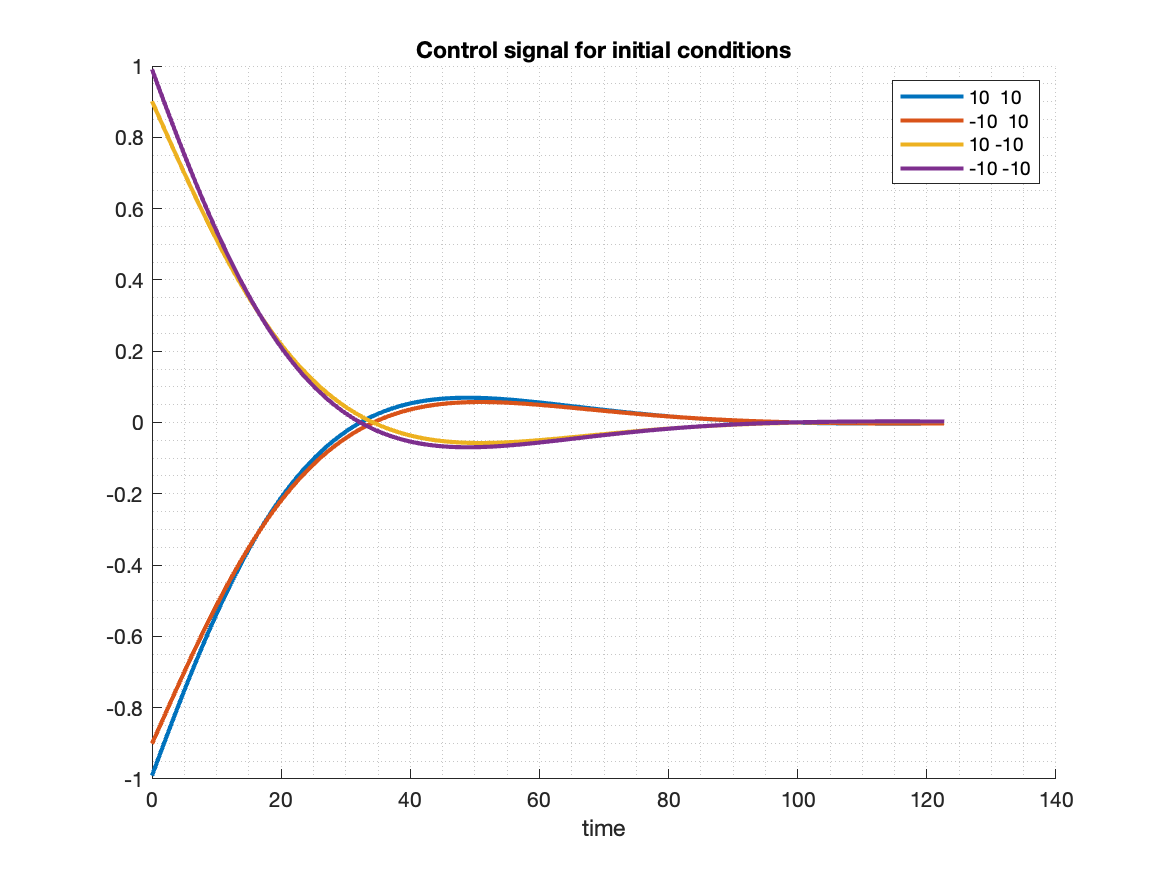
\includegraphics[width=0.8\textwidth]{plot1}
    \caption{Control signals for different initial conditions}
    \label{fig:plot1}
\end{figure}
